\section{解析}
\subsection{フィッティングの範囲指定}
今回の測定で得られたデータを$\mu$粒子が崩壊してできた電子のシンチレータへの到達時間[ns]を‎横軸に、各到達時間のイベント数を縦軸に示してフィッティングをするが、$\mu^-$は$\mu^+$より非常に短い寿命を持つ(1.1参照)ことから1000ns以下では$\mu^-$に対応する減衰曲線が無視できないと判断して1000ns以降からのデータを用いてフィッティングすることにした。

\subsection{寿命の解析}
実験aで得られたデータを1000nsから20000nsの範囲をビン数300でヒストグラムにし、それに対して関数
\begin{equation}
F(t)=A\exp\left(-\frac{t}{\tau}\right)+B
\end{equation}
でフィッティングを行う。ただし、$A,B$は定数、$\tau$は寿命である。
%% その結果を図\ref{}に示す。
\begin{figure}[htbp]
  \centering
  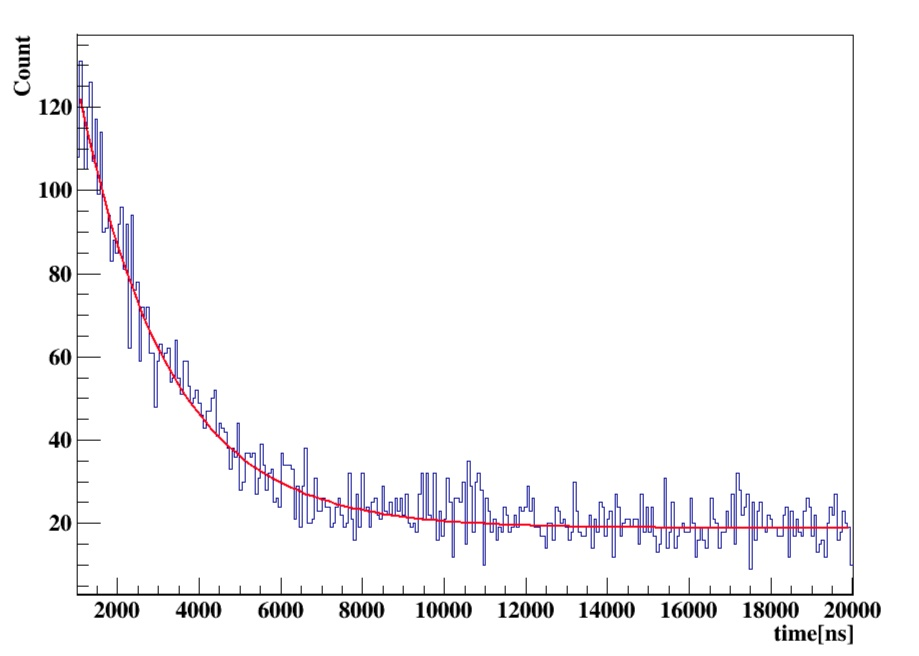
\includegraphics[width=10cm,bb=0 0 919 656]{lifetime.jpg}
  \caption{$\mu$の寿命曲線}
  \label{実験aのフィッティング}
\end{figure}

この結果、
\begin{align}
A &= 170 \pm 7  \\
B &= 18.8 \pm 0.4 \\
\tau &= 2.19 \pm 0.08\,\mathrm{\mu s}
\end{align}
を得た。このフィッティングにおける$\chi^2/\mathrm{ndf}$は1.00231であった。

\subsection{$g$因子の解析}
%%測定で出たデータを図\ref{}に示す。
%% \begin{figure}
%%  \centering
%%  \includergraphics[width=5cm,clip]{}
%%  \caption{$g$因子測定のヒストグラム}
%%  \label{}
%% \end{figure}

このヒストグラムに対し、関数
\begin{equation}
G(t)=A\exp\Bigl(-\frac{t}{\tau}\Bigr)(1+B\cos(\omega(t-t_0)))+C
\end{equation}
でフィッティングを行う。ただし、$A,B,C$は定数、$\tau$は寿命、$\omega$はスピンの歳差運動の振動数、$t_0$は初期位相を考慮した定数である。これは$\mu$粒子が磁場の影響で歳差運動を起こし(1.3参照)、その結果崩壊後飛び出す電子の運動の向きが変わることを考慮した。
%% その結果を図\ref{}に示す。

%% \begin{figure}
%%  \centering
%%  \includergraphics[width=5cm,clip]{}
%%  \caption{$g$因子測定の寿命曲線}
%%  \label{}
%% \end{figure}

この結果、
\begin{equation}
A= ,B= ,C= ,\tau= ,\omega= ,t_0=
\end{equation}
を得た。
